\lecture{Interconnections}{2023-02-13}{16:00}{Farzad}{RB LT1}

\section{Interconnection Structure}
Computers are a network of basic modules, connected together by paths (such as the system bus). The structure of these paths depends on the exchanges taking place.

\subsection{Memory}
Within memory there are n-words, each of equal length. Each word has a unique numerical address. The operation which the memory is currently performing is controlled by read and write control signals. The location for the operation is specified by an address. Data can be written to or read from memory.

\subsection{Input/ Output Module}
The Input/ Output (I/O) Module is similar to memory from an internal point of view, in that data can be read-from and written-to it. The I/O module can control more than one external device (each port has a unique address which can be used to identify an individual device). The I/O module has internal data input and output ports, this is for data coming from/ going to other places inside the computer; it also has external data in and out ports, which are used for interfacing with an external device. The I/O module also has the ability to send interrupt signals to the CPU which signals to the CPU to stop doing what it was doing as something more important has happened (for example, printer has run out of paper) which it needs to deal with.

\subsection{Processor}
The processor reads instructions and data and writes out data after processing. It uses control signals to control the overall operations. The processor also receives interrupt signals.

\subsection{Types of Transfer}
\begin{description}
    \item[Memory to Proecssor] The processor reads an instruction or unit of data from memory
    \item[Processor to Memory] The processor writes a unit of data to memory
    \item[I/O to Processor] The processor reads data from an I/O device via an I/O module
    \item[Processor to I/O] The processor sends data to the I/O device
    \item[I/O to or from Memory] I/O module is allowed direct access to the memory rather than going through the CPU.
\end{description}

\section{Bus Interconnection}
Bus interconnections are not used much in modern systems as they are a shared transmission medium which means there is only a single route which all data must travel on. Multiple devices connect to the bus and a signal transmitted by one device is available for reception by all other devices attached to the bus. If signals overlap, they become garbled therefore only one device at a time can successfully transmit. A bus consists of multiple communication pathways (called lines); each transmits a single bit at a time which means if we want to transmit 8-bits simultaneously, we need a bus with a bus-width of 8. 
\begin{figure}[H]
    \centering
    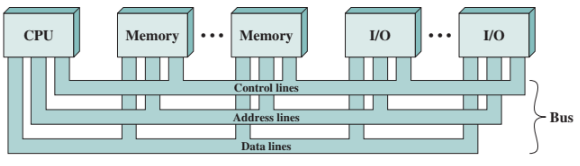
\includegraphics[width=0.9\textwidth]{assets/bus-interconnection.png} 
    \caption*{Bus interconnections}
\end{figure}
\subsection{Data Lines}
The data lines provide a path for moving data among system modules. The width of the data bus is a key factor in determining overall system performance. For example, if the data bus is 32 bits wide and the instruction to be transmitted is 64-bits then you need to use the data bus twice whereas if the data bus was 64-bits wide then you would only need to use it once.

\subsection{Address Lines}
The address bus carries the source/ destination of the data which is being transmitted on the data bus. The bus width determines the maximum possible memory capacity. Typically, the high order bits select the module on the bus and the low order bits select the memory location or I/O port.

\subsection{Control Lines}
Control lines control the access to and use of the data and address lines because the data and address lines are shared by all components and there must be a means to control their use. Control signals are transmitted on control lines, these include command signals which specify the operation to be performed and timing signals which confirm the validity of data and address information. Control lines include memory write \& read, I/O write \& read etc.

\subsection{Bus Operation}
If one module wishes to send data to another, it must first obtain use of the bus then it can transfer the data via the bus.

If one module wishes to request data from another module, it must first obtain the use of the bus. Then it can transfer a request to the other module over the appropriate control and address lines. 

\section{Point-To-Point Interconnection}
Contemporary systems increasingly rely on point-to-point interconnections. This removes the bus system problems as well as lowering the latency, increasing the data rate and improving the scalability.
\subsection{QuickPath Interconnect}
QuickPath Interconnect (QPI) was released in 2008. It includes multiple direct connections, a layered protocol architecture and packetized data transfer.

\begin{figure}[H]
    \centering
    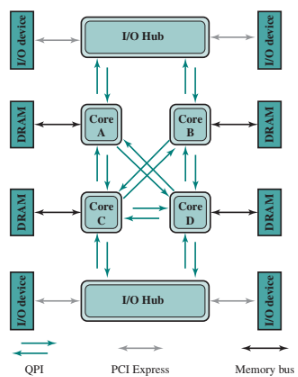
\includegraphics[width=0.4\textwidth]{assets/qpi.png} 
    \caption*{Point-To-Point Interconnection diagram showing QuickPath}
\end{figure}